\documentclass{article}
\usepackage[usenames,dvipsnames]{color} % Required for custom colors
\usepackage{graphicx} % Required to insert images
\usepackage{listings} % Required for insertion of code
\usepackage{amsmath} % Required for some math formulas
\usepackage{enumitem} % Required for customed enum
\usepackage{url} % Auto line break in URL
%\usepackage{tabularx} % Auto line break in tabular
\usepackage{ltablex} % Required for auto page break tabular
\usepackage{booktabs} % Required for table
\usepackage{dirtree} % Required for directory tree

\def\UrlBreaks{\do\[\do\\\do\]\do\^\do\_\do\`\do\.\do\@\do\\\do\/\do\!\do\_\do\|\do\;\do\>\do\]\do\)\do\,\do\?\do\'\do+\do\=\do\#}

\usepackage{hyperref} % add clickable link to contents
\hypersetup {
    colorlinks = false, % links colored or not
    hidelinks = true, % border
    linkcolor = blue, % color TOC links in blue
    urlcolor = red, % color URLs in red
    linktoc = all % 'all' will create links for everything in the TOC
}

% Uncomment the lines below if you wish to use Chinese characters
\usepackage{fontspec}  % Chinese characters support
\usepackage{indentfirst} % Add indent at the first paragraph
\XeTeXlinebreaklocale "zh" % Automatic line break
\XeTeXlinebreakskip = 0pt plus 1pt % Automatic line break
% \setmainfont{STSong} % Use a Chinese font
% \setmainfont[Path = ./]{AdobeSongStd-Light.otf} % use font in ./
\setmainfont[Path = fonts/]{AdobeFangsongStd-Regular.otf}

% Use Chinese for figure name
\renewcommand\figurename{图}

% Use Chinese for contents name
\renewcommand\contentsname{目录}

% Use Chinese for table name
\renewcommand\tablename{表}

% contents depth
\setcounter{tocdepth}{2}

% numbered paragraph
\setcounter{secnumdepth}{4}

%----------------------------------------------------------------------------------------
%	TITLE SECTION
%----------------------------------------------------------------------------------------

\newcommand{\horrule}[1]{\rule{\linewidth}{#1}} % Create horizontal rule command with 1 argument of height

\title{	
\normalfont \normalsize 
% \textsc{university, school or department name} \\ [25pt] % Your university, school and/or department name(s)
\horrule{0.5pt} \\[0.4cm] % Thin top horizontal rule
\huge Cache Debugger技术文档 \\ % The assignment title
\horrule{2pt} \\[0.5cm] % Thick bottom horizontal rule
}

\author{Cache小组} % Your name

\date{\normalsize\the\year 年\the\month 月\the\day 日} % Today's date or a custom date




% document begin
\begin{document}
\maketitle % Print the title

\tableofcontents % Print the contents

\newpage % blank after contents

\section{引言}
    \subsection{开发信息}
        系统名称:硬件调试工具Cache Debugger

        开发者:
        \begin{minipage}[t]{0.8\linewidth}
        计23 李天润

        计23 胡津铭

        计23 孙皓
        \end{minipage}

    \subsection{内容简介}
        本文档介绍了硬件调试工具的功能设计以及软硬件部分实现细节,方便读者更深入了解本工具的运行方式,以及根据自己的需要对工具进行修改、开发。

        本文档假设读者已经阅读过调试工具的使用手册,并且了解硬件描述语言的基本应用以及元件例化的方法。

\section{设计原理}
    硬件逻辑分时序逻辑与组合逻辑,其中组合逻辑仅与输入有关,时序逻辑受时钟控制。

    在系内课程与FPGA有关的实验中,并没有涉及与延时相关的逻辑,比如振荡电路,因此FPGA芯片内部的硬件延时在设计硬件逻辑时一般不会被考虑,仅影响时钟频率的提高。%
    基于以上考虑,可以认为大多数实验中,硬件逻辑的执行是由时钟驱动的,因此控制了时钟也就控制了逻辑的执行。%
    而且,由于设计逻辑时不会将延时作为正面的逻辑功能的一部分,时钟沿无论延迟多久到达都不会产生负面作用,因此暂停时钟相当于将电路暂停,之后再次给入时钟信号即可无损地继续执行程序。

    本工具正是基于以上结论,结合调试的断点信息,产生被调试模块的时钟信号,使得被调试模块既可正常运行,又可以在给定的状态下暂停,查看调试信息。

    通过逻辑操作,本工具可以为被调试模块提供与调试工具的输入时钟信号相同频率的时钟信号,使得被调试模块在调试环境下有着与实际单独运行时几乎相同的表现。

\section{硬件部分}
    \subsection{整体设计}
        硬件部分,需要在软件客户端的控制下,产生适当的时钟信号,控制程序运行指定的时钟数或者运行到指定的断点状态。

        运行结束之后,应当将硬件上的信号值发送到客户端,以供调试人员查看信号值,分析芯片运行状况。

        调试工具的硬件部分工作流程如图\ref{process}。

        \begin{figure}[htbp!]
            \centering
            \caption{硬件部分工作流程示意图}\label{process}
            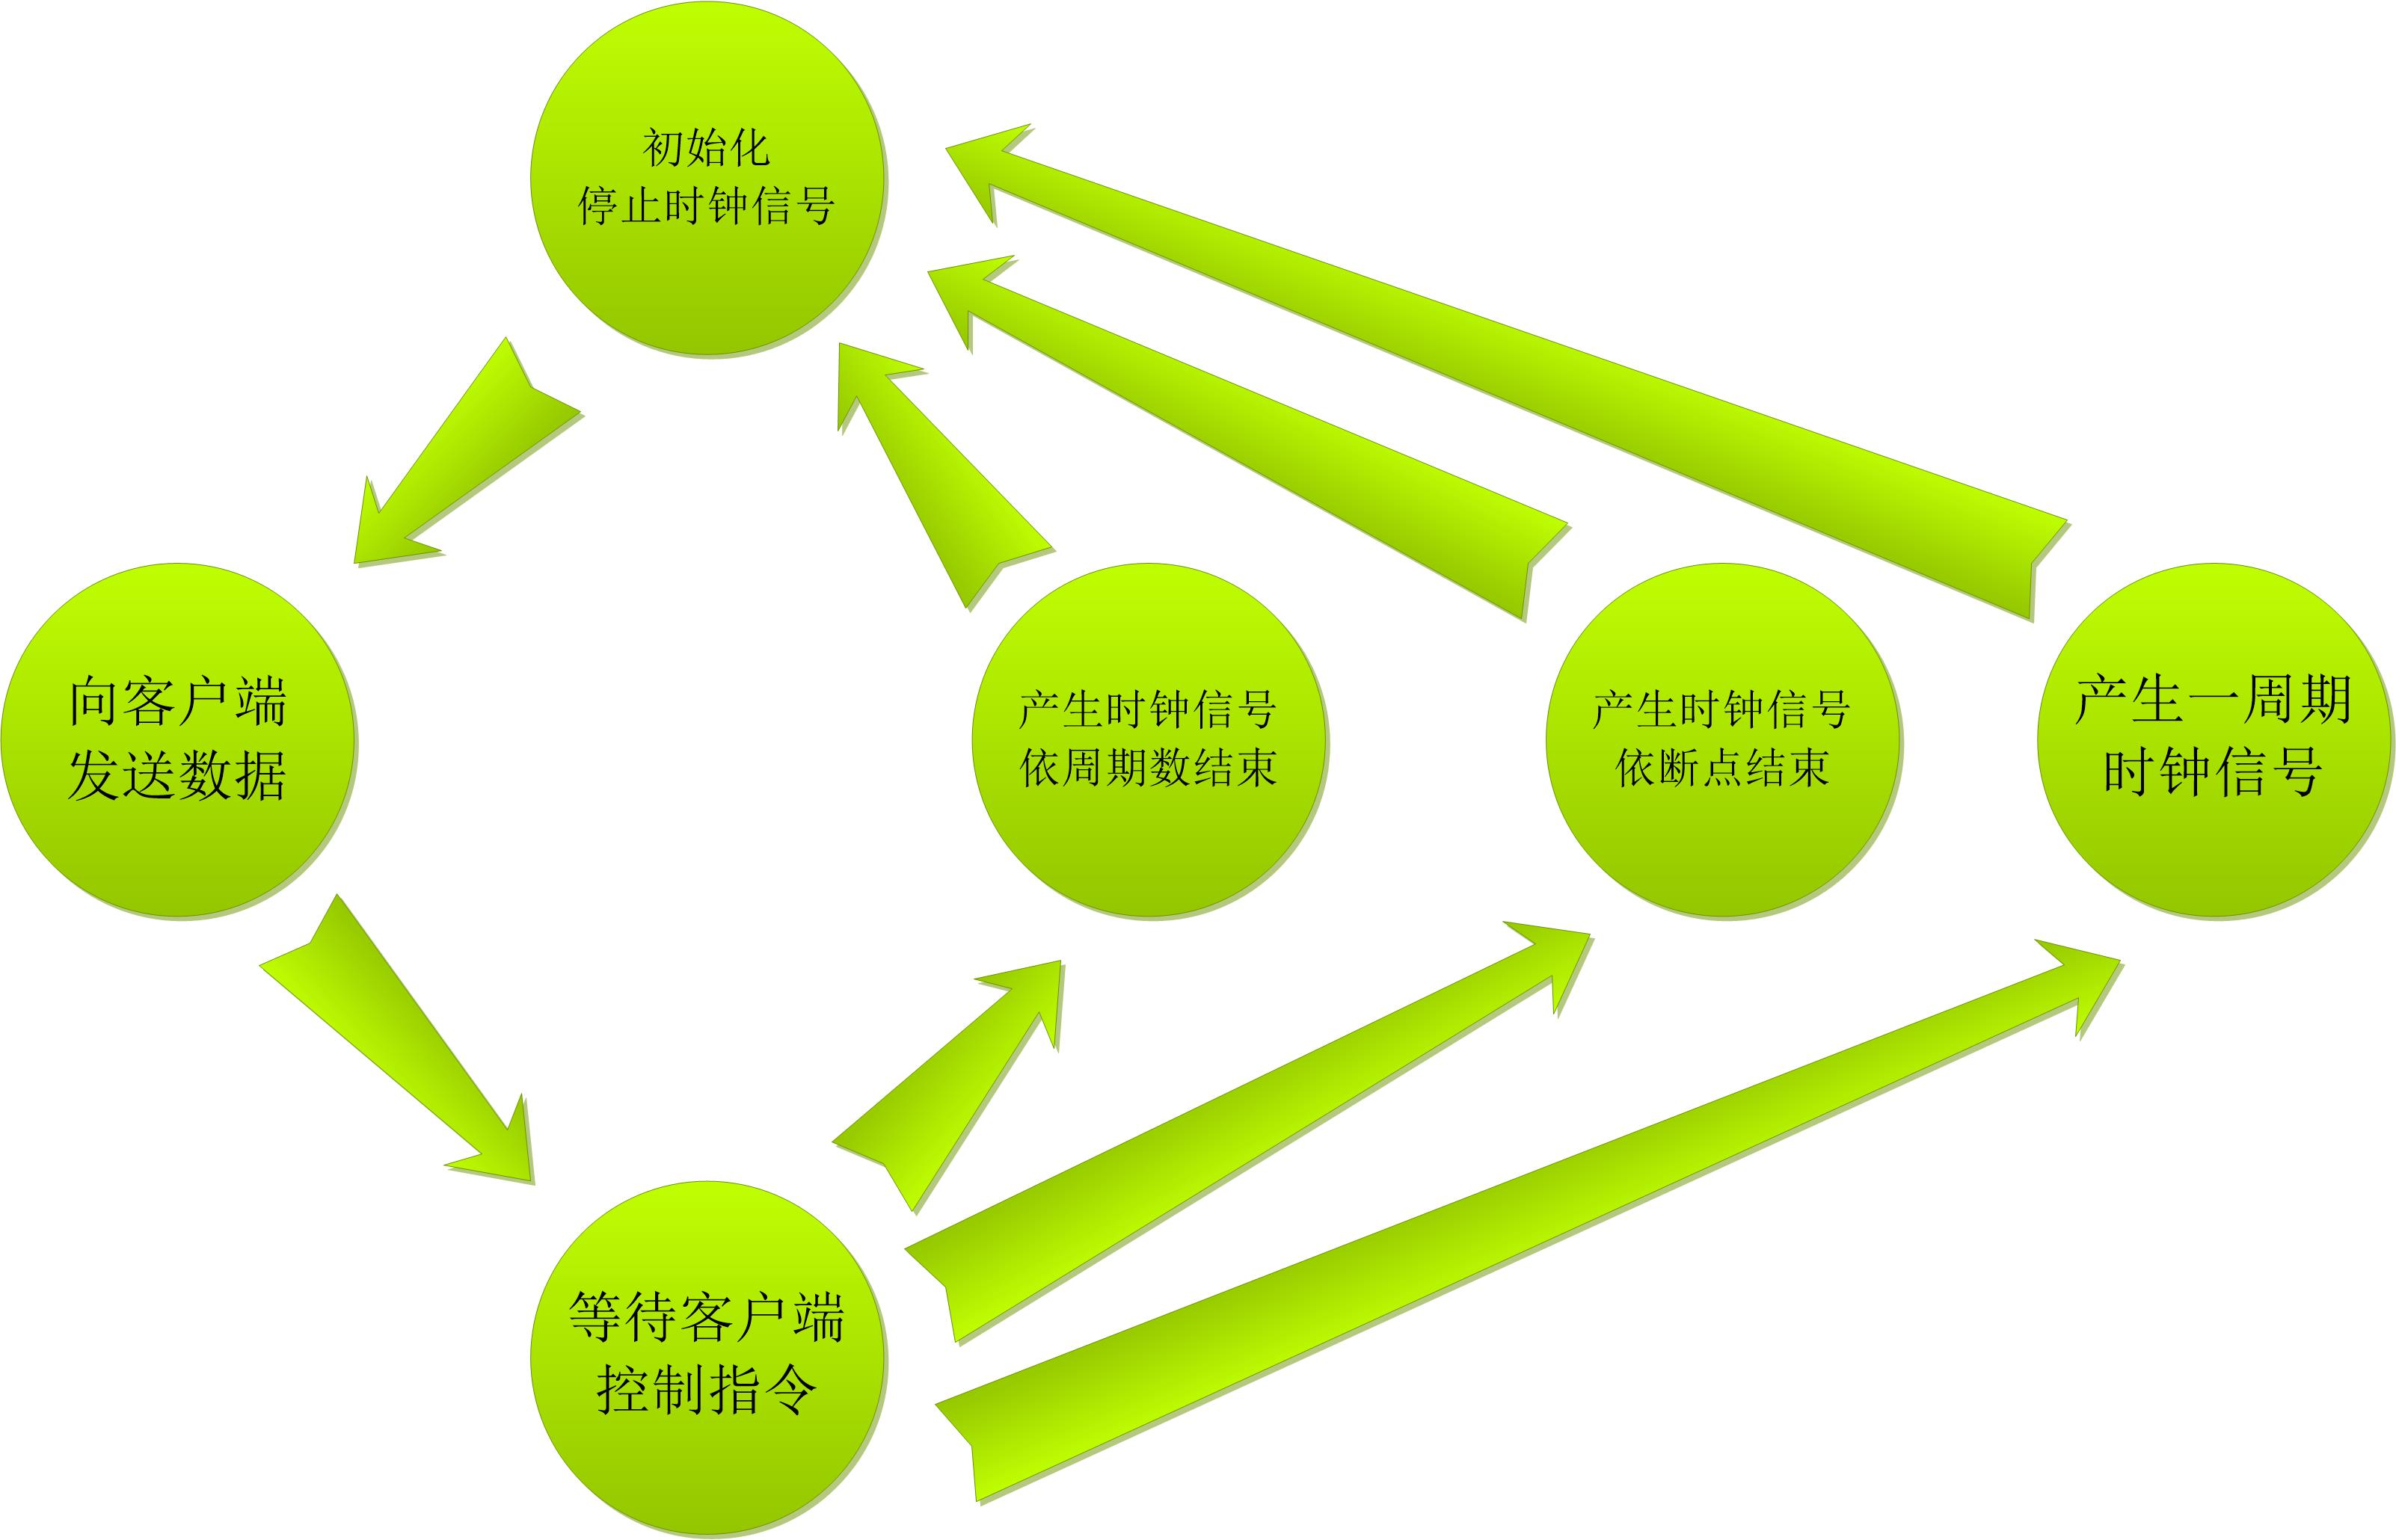
\includegraphics[width=0.5\textwidth]{chart/hardware_path.jpg}
        \end{figure}

        上述功能由两个模块实现,一个模块用于与客户端进行通信,另一个模块用于控制被调试模块的时钟信号以及调试工具的状态跳转。
    \subsection{模块设计}
        \subsubsection{控制模块}
            此模块位于bp\_debug.vhd

            \paragraph{端口说明}
            \mbox{}
                        \begin{tabularx}{\textwidth}{lll}
            \toprule
            端口名          & 端口方向  & 端口类型 \\
            \cmidrule(l){2-3}
            &
            \multicolumn{2}{X}{端口描述} \\
            \midrule
            clk             & in        & std\_logic \\
            \cmidrule(l){2-3}
            &
            \multicolumn{2}{X}{
                时钟输入。
            } \\
            \midrule
            clk\_o             & out        & std\_logic \\
            \cmidrule(l){2-3}
            &
            \multicolumn{2}{X}{
                由此模块产生的时钟信号,可直接作为被测试模块的时钟。
            } \\
            \midrule
            e             & in        & std\_logic \\
            \cmidrule(l){2-3}
            &
            \multicolumn{2}{X}{
                使能信号。
            } \\
            \midrule
            datas             & in        & std\_logic\_vector ( 4095 downto 0 ) \\
            \cmidrule(l){2-3}
            &
            \multicolumn{2}{X}{
                从被测试模块发来的信号值数据。
            } \\
            \midrule
            monitor             & in        & std\_logic\_vector ( 63 downto 0 ) \\
            \cmidrule(l){2-3}
            &
            \multicolumn{2}{X}{
                从被测试模块发来的监控信号数据,用于断点的监控。
            } \\
            \midrule
            serialport\_txd        & out      & std\_logic \\
            \cmidrule(l){2-3}
            &
            \multicolumn{2}{X}{
                串口写端口。
            } \\
            \midrule
            serialport\_rxd             & in        & std\_logic \\
            \cmidrule(l){2-3}
            &
            \multicolumn{2}{X}{
                串口读端口。
            } \\
            \bottomrule
        \end{tabularx}


            \paragraph{内部实现}
            \mbox{}

                控制模块的状态机大致与调试工具硬件部分的工作流程相对应。

                需要查看的信号值部分,从被调试模块获取信号值(默认长度为4096bit),使用组合逻辑的方法根据通信模块给出的字节编号选取对应的字节提供给通信模块。

                调试部分,目前仅支持在上升沿之前断点,实现方式为输出时钟由两个中间值取异或得到。%
                一个中间值的改变由输入时钟下降沿触发,在输出时钟为高电平时对其取反。%
                令一个中间值的改变由输入时钟上升沿触发,在程序运行阶段,且仍需继续运行时,如果输出时钟为低电平,则将其取反。

                被调试模块是否应当继续运行,根据指令的不同而有不同的判断方式。

                对于断点调试而言,当检测信号与段电信号值相同时应当进行停止运行,否则应当继续运行。

                对于继续调试而言,应当无条件给出一个周期的时钟信号,然后按照断点调试判断。

                对于单步调试而言,设置一个倒计时计数器,每次时钟上升沿减一且被调试模块运行,减到0时被调试模块停止运行。

        \subsubsection{通信模块}
            此模块位于com\_debug.vhd

            \paragraph{端口说明}
            \mbox{}

                        \begin{tabularx}{\textwidth}{lll}
            \toprule
            端口名          & 端口方向  & 端口类型 \\
            \cmidrule(l){2-3}
            &
            \multicolumn{2}{X}{端口描述} \\
            \midrule
            clk             & in        & std\_logic \\
            \cmidrule(l){2-3}
            &
            \multicolumn{2}{X}{
                串口发送部分开始信号。
            } \\
            \midrule
            slc             & out        & std\_logic\_vector(15 downto 0) \\
            \cmidrule(l){2-3}
            &
            \multicolumn{2}{X}{
                串口发送的字节编号,用于从上层模块获取对应字节。
            } \\
            \midrule
            data             & in        & std\_logic\_vector ( 7 downto 0 ) \\
            \cmidrule(l){2-3}
            &
            \multicolumn{2}{X}{
                串口发送的字节值,使用编号slc从上层模块获取。
            } \\
            \midrule
            serialport\_txd        & out      & std\_logic \\
            \cmidrule(l){2-3}
            &
            \multicolumn{2}{X}{
                串口写端口。
            } \\
            \midrule
            serialport\_rxd             & in        & std\_logic \\
            \cmidrule(l){2-3}
            &
            \multicolumn{2}{X}{
                串口读端口。
            } \\
            \midrule
            data\_coming             & out        & std\_logic \\
            \cmidrule(l){2-3}
            &
            \multicolumn{2}{X}{
                标志位,表示客户端指令到来。
            } \\
            \midrule
            coming\_data             & out        & std\_logic\_vector ( 135 downto 0 ) \\
            \cmidrule(l){2-3}
            &
            \multicolumn{2}{X}{
                来自客户端的指令信息。
                高64位为客户端第二个参数;
                中64位为客户端第一个参数;
                低8位表示指令类型。
            } \\
            \midrule
            data\_read             & in        & std\_logic \\
            \cmidrule(l){2-3}
            &
            \multicolumn{2}{X}{
                标志位,表示这一指令已经被读取,可以消除指令到来信号。
            } \\
            \bottomrule
        \end{tabularx}


            \paragraph{内部实现}
            \mbox{}

                通信模块包括接受与发送两部分,分别工作,相互不影响,通过软件端、控制模块保证发送与接受的顺序。

                发送部分用于运行结束时,向客户端发送需要的内部信号值。%
                收到控制端的发送开始信号后,从0号字节开始循环发送。%
                这一部分使用slc端口给出字节编号,然后由data读入字节信息,通过串口发送。

                接收部分从软件端接受指令,收到17个字节后,通过标志位通知控制模块数据到来,同时提供数据。%
                收到控制模块读走数据的信号后,接收部分将数据到来标志位清零,同时继续等待新数据到来。

                此部分工作频率默认在50MHz,%
                频率不符会导致此部分不能正常工作。%
                修改频率请在async.v中做修改。


\section{软件部分}
    \subsection{设计原理}
        软件端设计与硬件端匹配,与硬件端约定接收、发送规则,%
        接收、发送消息的格式,%
        同时为了解决数据传输过程中可能出现的错误,%
        还需要处理系统缓冲区、检测丢包现象,%
        从而保证调试工具正常运行。%
    \subsection{整体设计}
        软件端开始运行后读取配置文件,尝试连接串口,%
        以上操作均成功后,进入用户操作界面。
            
        \subsubsection{通信命令编码}
            对于每个用户输入的命令,软件端将命令编码后发送给硬件端,%
            根据命令类型决定是否阻塞并等待硬件端数据。

            通信编码共17字节,命令编码规则如下表所示。%
            图中编码低序字节最先发送,高序字节最后发送。

            \begin{tabularx}{\textwidth}{llX}
                \toprule
                命令 & 通信编码 & 说明 \\
                \midrule
                run        & 0x<128位全0>01 & 运行此命令后软件端阻塞,等待硬件端数据。 \\
                \midrule
                break      & 0x<64位掩码><64位数据>02 & 64位数据为断点条件,%
                                                        掩码为1表示数据有效,%
                                                        掩码为0表示数据通配,%
                                                        数据和掩码均采用小端法。 \\
                \midrule
                continue   & 0x<128位全0>03 & 运行此命令后软件端阻塞,等待硬件端数据。 \\
                \midrule
                step       & 0x<64位全0><64位数据>04 & 64位数据为前进时钟数,%
                                                       运行此命令后软件端阻塞,%
                                                       等待硬件端数据。 \\
                \midrule
                print      & & 此命令无需与硬件端通信。 \\
                \midrule
                display    & & 此命令无需与硬件端通信。 \\
                \midrule
                undisplay  & & 此命令无需与硬件端通信。 \\
                \midrule
                help       & & 此命令无需与硬件端通信。 \\
                \midrule
                quit       & & 此命令无需与硬件端通信。 \\ 
                \bottomrule
            \end{tabularx}

        \subsubsection{通信数据编码}
            软件运行后会自动读取当前目录下cadb.cfg文件。%
            配置文件需要用户自行编写,共三列,%
            第一列是软件端查看变量值时的标签,接受不包含空白字符的字符串。
            第二列是VHDL源代码中实际被查看信号名称,%
            接收不包含空白字符的字符串,在被调试模块中应有同名信号,%
            且该信号不能为输出端口。
            第三列是被查看信号的范围。%
            对于std\_logic\_vector应标明范围,%
            对于std\_logic第三列置空。

            生成VHDL代码时,程序会根据信号长度在通信数据格式中从低到高分配,%
            对于长度不是8的整数倍的信号,会填充0以实现8对齐。%
            每次收到硬件端发送的数据后,软件端会根据该格式解析出对应的信号值。%
            因此每次修改配置文件后都应该重新生成VHDL代码并应用到硬件中。%
            数据在传输和保存过程中采用小端法,%
            因此在打印变量时从高序字节开始打印。

            若要修改通信数据总长度,%
            应在软件端源代码中修改类Parser的静态成员常量MSG\_LENGTH的值,%
            同时在硬件端做相应修改。%
            注意该值在软件端以字节为单位,在硬件端以位为单位。

        \subsubsection{系统缓冲区管理}
            Unix操作系统中为串口设置有缓冲区,%
            缓冲区大小因操作系统不同而有所差异。%

            为了避免软件运行过程中受缓冲区原有数据影响而造成通信不同步,%
            软件启动时和run命令发送之前应清空系统缓冲区。%
            清空方法为:不断尝试读取串口,直到连续10ms读取不到数据为止。

        \subsubsection{丢包检测}
            在软硬件两端通信协议设置正确且%
            硬件运行过程中能够到达断点条件的前提下,软件端一直阻塞,%
            则说明发生了串口传输丢包现象。%
            此时应重启软件端。

            本工具自开发使用以来从未发现丢包现象。
        \subsubsection{串口通信参数}
            软件端串口通信管理在源代码类Communicator中,%
            如果需要修改波特率等串口通信参数,请在硬件端和软件端同时修改。
        

\section{高级应用}
    此部分涉及较多细节,请在理解本文档前述部分之后再进行阅读。
    \subsection{断点调试}
        本调试工具的断点调试可以按照64位均匹配的方式执行,也可以根据需要进行一定的通配匹配。

        对于包含通配符的断点信息,来自客户端的指令的第二个参数不再是0xFFFFFFFF,而在需要通配的位上为0。%
        断点的匹配是将断点值与监控值作异或,如果结果为0x00000000,则表示到达断点。%
        考虑通配符后,异或的结果会再与通配值进行与操作,将被设为通配的位置0,从而使其不再参与断点匹配。

    \subsection{观察信号变长}
        默认文件中,观察信号长度为4096bit,使用中可以将CPU顶层模块的所有信号以及通用寄存器、CP0寄存器的所有信号发到客户端,
        而且发送这一长度的观察信号消耗的时间在通过终端查看的情况下可以忽略。

        使用中,考虑到不同的使用者可能有不同的需要,比如自动调试中希望每次发送更少的信号值或者需要发送更多的信号,在此给出改变观察信号长度的方法。

        % 不必须
        % 需要注意的是,数据发送以字节为单位,因此需要保证观察信号的长度为8的倍数。

        改变观察信号长度,需要将被调试模块中的输出数据长度改变,调试模块的输入数据长度改变。

        接下来,需要将数据发送部分的字节编号范围改为需要的数值,此处需修改com\_debug.vhd中的常量slc\_max。

        最后,需要在软件端进行相应修改,使其一次性接受的信号数量匹配。


\end{document}
